\vspace{-0.1cm}
\section{Proposed Pipeline}
\label{sec:proposed}

\begin{figure}
    \centering
    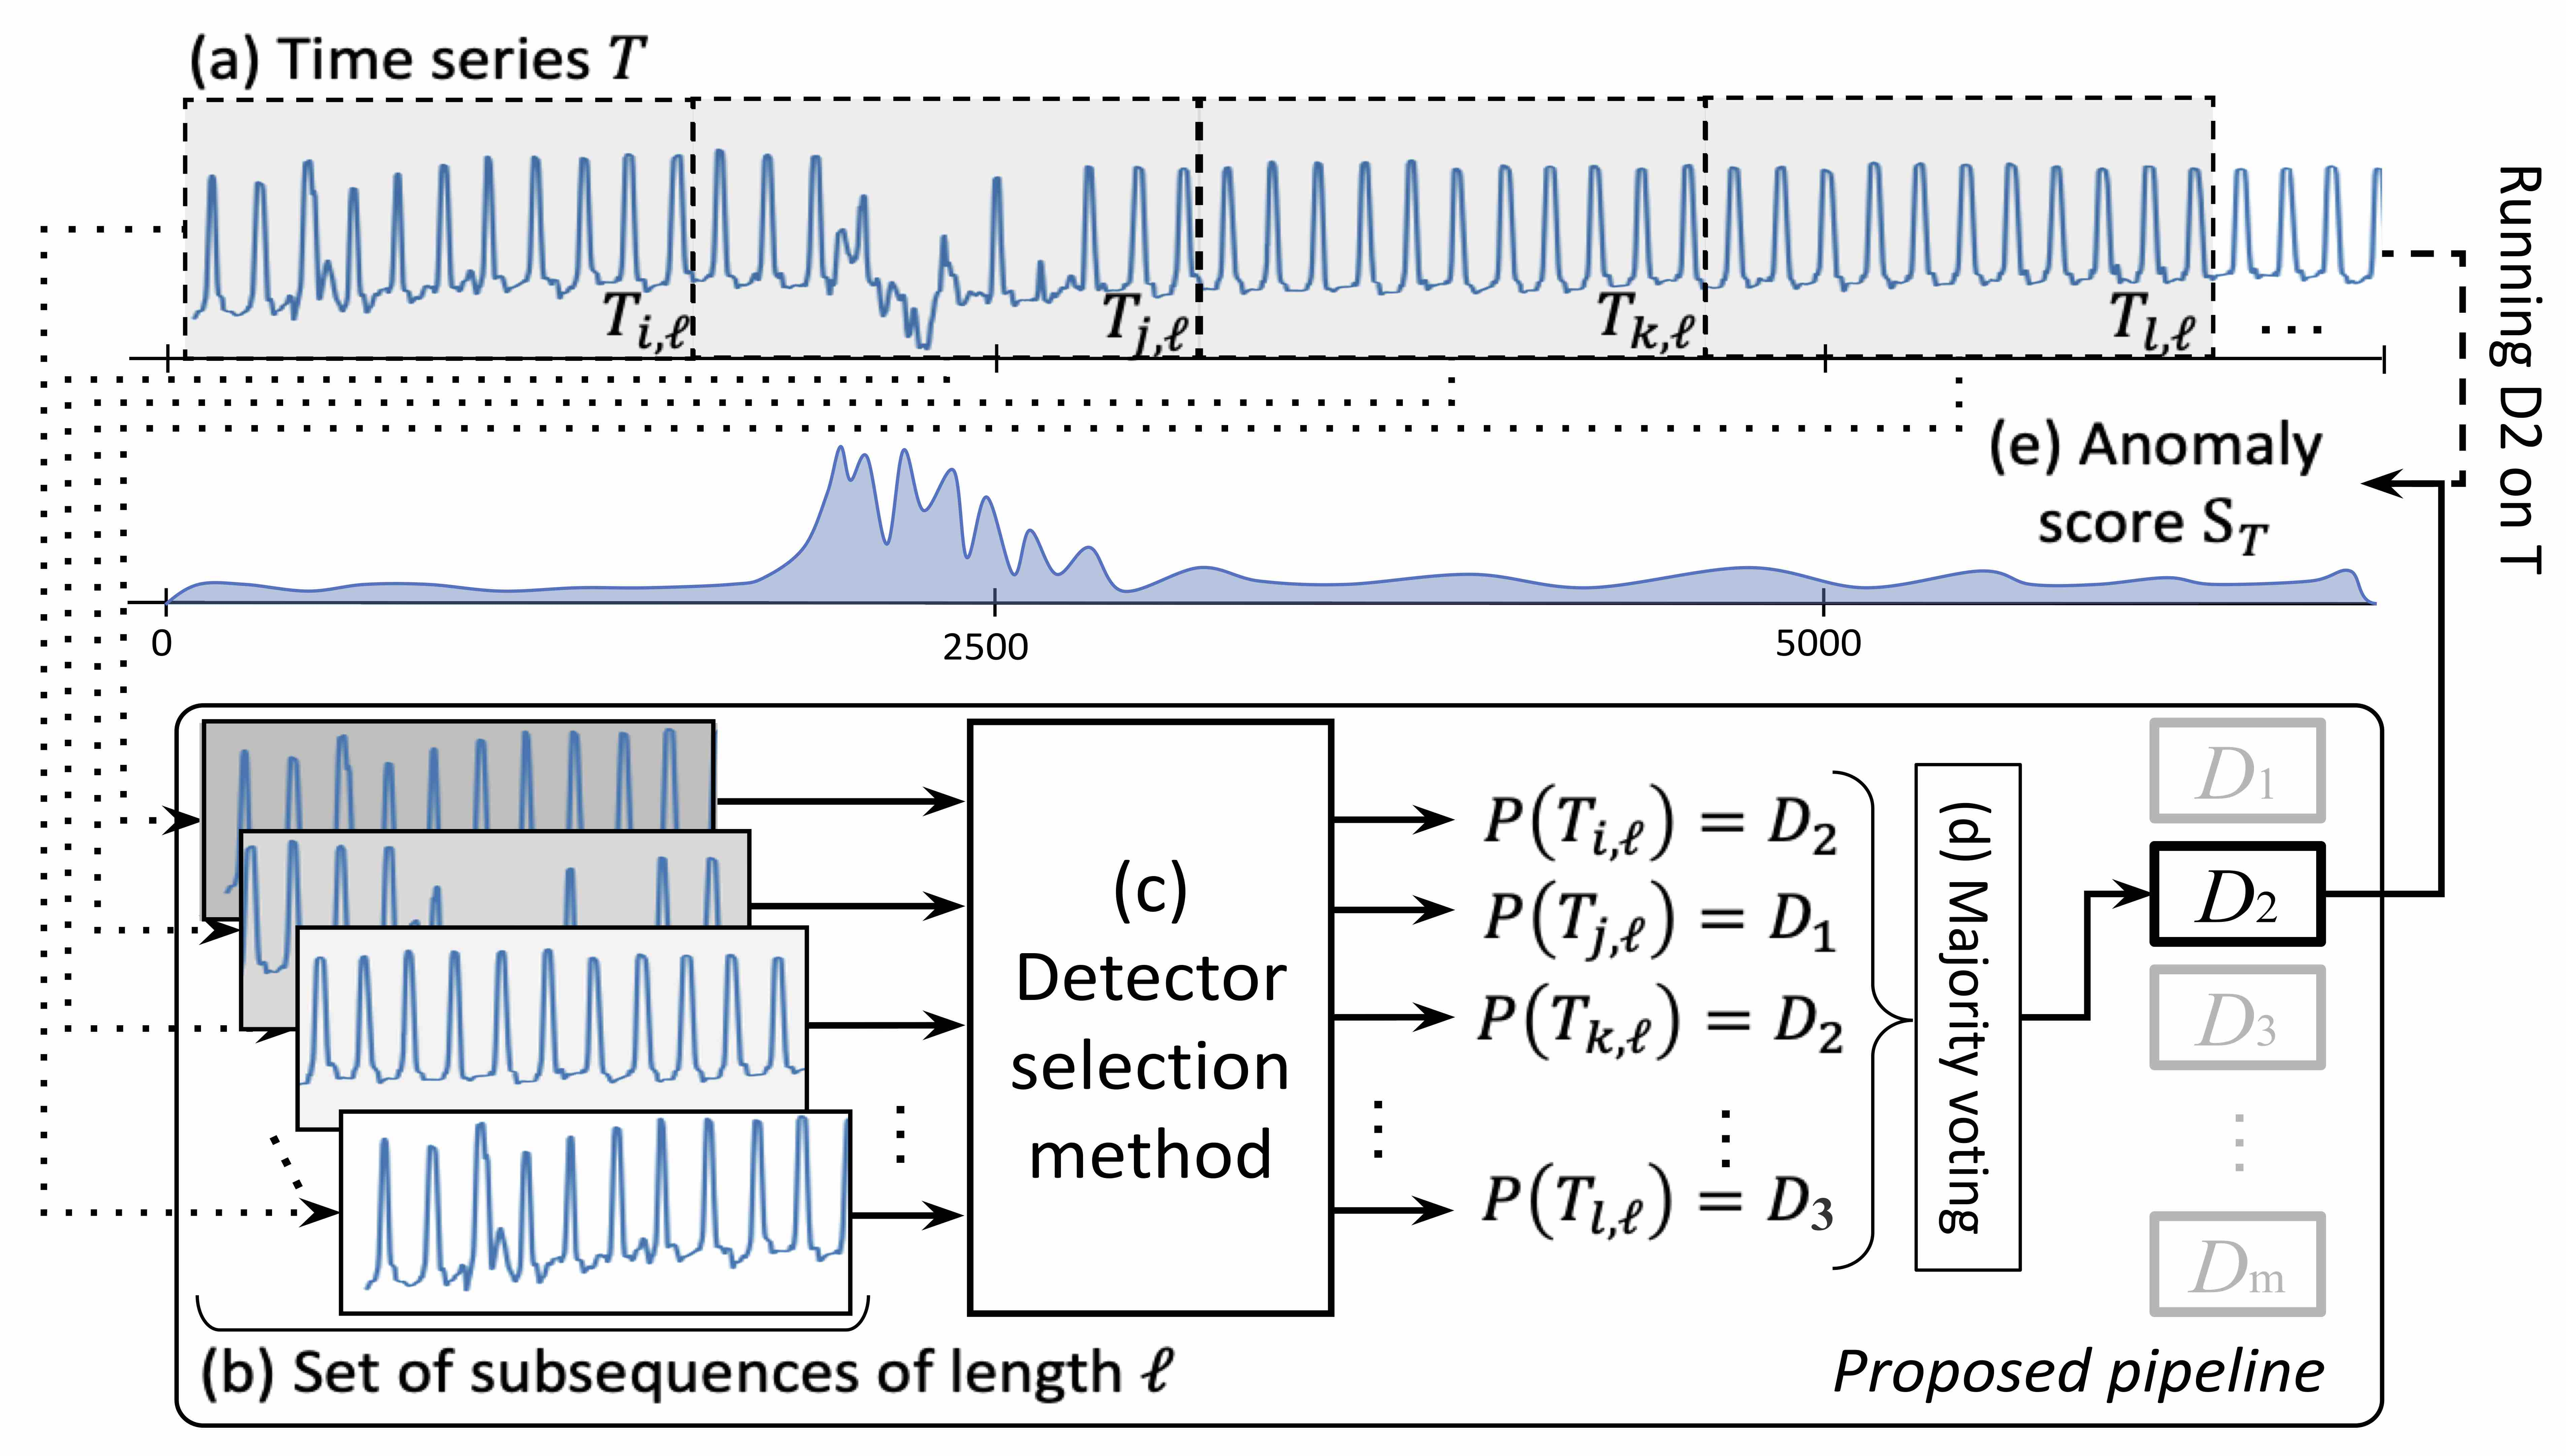
\includegraphics[width=0.94\linewidth]{figures/3_pipeline.jpg}
    \vspace{-0.3cm}
    \caption{Proposed pipeline for the method selection}
    \label{fig:proposed_work}
    \vspace{-0.3cm}
\end{figure}

In the following section, we provide a comprehensive explanation of the proposed pipeline. This pipeline corresponds to a sequence of preprocessing and postprocessing steps such that the inputs of the model selection algorithms are equal in length. The proposed pipeline, illustrated in Figure~\ref{fig:proposed_work}, is composed of the following steps: (i) \textbf{Preprocessing step}: Extraction of the subsequences of same lengths (Figure~\ref{fig:proposed_work} (b)), (ii) \textbf{Prediction step}: Prediction of which detector to use for each subsequence (Figure~\ref{fig:proposed_work} (c)), and (iii) \textbf{Selection step}: Majority voting among all the different prediction to select one detector only (Figure~\ref{fig:proposed_work} (d)). In the following section, we describe the three steps mentioned above in detail.

\vspace{-0.1cm}
\subsection{Preprocessing Step}
Time series classification can be performed with three different strategies: (i) treating the entire time series as one sample, (ii) dividing the time series into overlapping subsequences, (iii) dividing the time series into shifting subsequences (i.e., non-overlapping subsequences). The first strategy is straightforward, as each time series is treated as a single observation. Nevertheless, not all classifiers can handle variable-length inputs, and training such models can be computationally intensive (i.e., batches of time series cannot be treated in parallel). The second strategy involves dividing the time series into overlapping subsequences (of a given window length $\ell$). Despite possible loss of information, it forces each input of the methods to be the same length ($\ell$), allowing simpler and faster computation when performed in parallel. In the third strategy, we divide time series into non-overlapping subsequences (of a given length $\ell$), removing redundant information in overlapping subsequences. The latter might lead to separate anomalies into multiple windows, but significantly reduces the number of inputs generated by the second strategy and significantly accelerates the training and inference time. For these reasons, we chose the third strategy.

Thus, the time series of length $|T|$ are divided into $\mathbb{T}_l$ non-overlapping subsequences of length $\ell$. When the length of the time series is not divided evenly with the window length $\ell$, the remainder is added with an overlap between the first two windows. Formally, $\mathbb{T}_l$ is defined as follows:
\begin{equation*}
    \mathbb{T}_l = \left.
    \begin{cases}
        \big\{T_{i*\ell,\ell} \big| \forall i \in \big[0,\big\lceil \frac{|T|}{\ell} \big\rceil \big] \big\} &\text{, if } \big\lceil \frac{|T|}{\ell} \big\rceil = \frac{|T|}{\ell} \\
        \big\{ T_{0,\ell} \big\} \bigcup \big\{T_{|T| - \lceil \frac{|T|}{\ell} \rceil+i*\ell,\ell} \big| \forall i \in \big[0,\big\lceil \frac{|T|}{\ell} \big\rceil\big] \big\} &\text{, if } \big\lceil \frac{|T|}{\ell} \big\rceil < \frac{|T|}{\ell}
    \end{cases}
    \right. 
\end{equation*}
We expect the length $\ell$ to \syl{to have an impact on} the anomaly detection accuracy. We thus test multiple length values and measure their influence (on accuracy and execution time) in Section~\ref{sec:exp}.

At this point, we preprocessed the time series into subsequences of equal length. We now discuss the label (i.e., \syl{the} best detector to apply) attribution. For that matter, we use the TSB-UAD benchmark~\cite{10.14778/3529337.3529354} that contains 12 different anomaly detection methods. We compute the 12 methods for each time series and attribute the most accurate (based on AUC-PR) detector as the label. Then, the produced subsequences share the same label as the time series they originate from. This labeled dataset can be used to train classification methods and divided into the train, test, and validation sets. It is important to note that although each time series \syl{produces} multiple samples (i.e., subsequences), these samples should not be mixed between train, validation, and test set. Indeed, too strong similarities between subsequences that belong to the same time series, if contained in both the train, validation and the test, can lead the classification model to overfit or create an illusion of accuracy. Therefore, we guarantee that the intersection between the train, validation, and test set, regarding which time series the corresponding subsequences originate from, is empty.

\vspace{-0.1cm}
\subsection{Time Series Classification Approaches}

In this section, we describe the time series classifier approaches that we use as model selection methods. As many approaches have been proposed in the literature, we restrict our experimental evaluation to two main categories: (i) feature-based and (ii) raw-based methods. In addition, the second category can be divided into two sub-categories: (i) convolutional-based and (ii) transformer-based. %\syl{It is worth noting that raw-based methods also utilize features for classification, although the extraction of these features is performed automatically within the network. Despite this, we classify them as raw-based due to the nature of their input. }
Figure~\ref{fig:taxonomy} illustrates a simplified taxonomy of the methods considered, and we describe them in the following section.

\vspace{-0.1cm}
\subsubsection{Feature-based classification}
The main idea regarding feature-based classification is to use the dataset of time series (or subsequences of time series) to create a dataset whose samples are described by features common to all samples. Using the feature-based dataset, we then employ traditional machine learning classifiers to classify each time series. We use the TSFresh~\cite{CHRIST201872} (Time Series Feature extraction based on scalable hypothesis tests) to extract each subsequence's features. The latter is used for automated time series feature extraction and selection based on the FRESH algorithm~\cite{christ2016distributed}. More specifically, it automatically selects relevant features for a specific task. This is achieved using statistical tests, time series heuristics, and machine learning algorithms. 
The TSFresh package provides three options for automated feature extraction, \syl{namely}, (i) \textit{ comprehensive}, (ii) \textit{ efficient}, and (iii) \textit{ minimal}. The first two options provide 700 hundred features and the latter provides only 9. For scalability reasons (the dataset transformation can reach millions of subsequences), we consider the \textit{minimal} option in this paper.

Moreover, the objective is not to evaluate Feature-based classifiers \textit{per se}, but rather to evaluate the ability of TSFresh to extract meaningful features for time series classification (and model selection for anomaly detection, in particular). In this paper, we consider the following classification approaches.

\noindent\textbf{[SVC]}
A Support Vector Classifier (SVC)~\cite{10.1145/130385.130401} is a classifier that maps instances in space in order to maximize the width of the gap between the classes. New instances are mapped into the same space and classified according to which side of the gap they fall. 

\noindent\textbf{[Bayes]}
The naive Bayes classifier~\cite{Zhang2004TheOO} uses Bayes' theorem to predict the class of a new instance based on prior probabilities and class-conditional probabilities. The prediction is made by computing the posterior probabilities for each class.

\noindent\textbf{[MLP]}
A Multi Layer Perceptron (MLP)~\cite{Hinton1989ConnectionistLP} is a fully connected (connections between every neuron) neural network.

\noindent\textbf{[QDA]}
A Quadratic Discriminant Analysis (QDA)~\cite{Geisser1964PosteriorOF} Classifier is a linear discriminant analysis algorithm. The prediction is made by computing the discriminant functions for each class.

\noindent\textbf{[AdaBoost]}
AdaBoost~\cite{10.5555/646943.712093} is a boosting ensemble machine learning algorithm for solving classification problems. It creates a sequence of weak classifiers, where each classifier is trained on a weighted sample of the dataset. The prediction is made by combining the predictions of all classifiers, weighted by their accuracy.

\noindent\textbf{[Decision Tree]}
A Decision Tree Classifier~\cite{Hunt1966ExperimentsII} is a tree-based method that represents a sequence of decisions based on the features of the dataset. To classify a new instance, the algorithm follows the decisions in the tree to reach a leaf node associated with a class.

\noindent\textbf{[Random Forest]}
A Random Forest Classifier~\cite{598994} is an ensemble machine learning algorithm that combines multiple decision trees, where each tree is built using a random subset of the features and a random sample of the data. The final class prediction for a new instance results from the aggregation of the predictions of all trees.

\noindent\textbf{[kNN]}
A kNN classifier~\cite{Fix1989DiscriminatoryA} is a method that classifies instances based on their distance to other instances in a training set. The algorithm assigns the new instances to the class with the most number of closest neighbors among the $K$ nearest data points. 

\vspace{-0.1cm}
\subsubsection{Raw-based classification}

Instead of using features to perform classification, the raw values of the time series can be used. Indeed, whereas features are efficient for homogenizing time series datasets (e.g., setting a constant number of features for variable length time series), it might hide important information in the shape of consecutive values. Thus, many approaches that use raw-values time series have been proposed.

\noindent\textbf{[Rocket]} Among the recent raw-values methods, MiniRocket~\cite{dempster2021minirocket} is one of the state-of-the-art time series classification methods. The latter consists of a feature extraction step and a classification step. More specifically, MiniRocket works by transforming input time series using a small, fixed set of convolutional kernels and using the transformed features to train a logistic regression classifier (using stochastic gradient descent). We refer to MiniRocket as Rocket.

\vspace{-0.1cm}
\subsubsection{Convolutional-based classification}

Convolutional-based approaches take as input raw-values of time series and have been shown to be accurate for time series classification~\cite{DBLP:conf/sigmod/BoniolMRP22}.

\noindent\textbf{[ConvNet]}
A Convolutional Neural Network (CNN) \cite{DBLP:journals/corr/OSheaN15} is a type of deep learning neural network widely used in image recognition that is specially designed to extract patterns through data with a grid-like structure, such as images, or time series. A CNN uses convolution, where a filter is applied to a sliding window over the time series. The ConvNet architecture proposed in~\cite{DBLP:journals/corr/WangYO16} is composed of three stacked Convolutional blocks followed by Global Average Pooling (GAP), and a Softmax activation function. Each Convolutional block is composed of a convolutional layer (used with a kernel length of $3$) followed by a batch normalization layer, followed by a ReLU activation function is applied.

\noindent\textbf{[ResNet]}
The Residual Network (ResNet) architecture~\cite{https://doi.org/10.48550/arxiv.1512.03385} was introduced to address the gradient vanishing problem encountered in large CNNs~\cite{simonyan2015a}. A ResNet is composed of several blocks connected together with residual connections (i.e., identity mapping). For time series classification, a ResNet architecture has been proposed in~\cite{DBLP:journals/corr/WangYO16}, and has demonstrated strong classification accuracy~\cite{fawaz2019deep}. It is the same architecture as the previously described ConvNet, with additional residual connections between convolutional blocks.

\noindent\textbf{[InceptionTime]}
The model consists of a network using residual connections and convolutional layers with kernels of variable lengths~\cite{fawaz2020inceptiontime}. Such a network uses \syl{three} Inception blocks that replace the traditional residual blocks that we can find in a ResNet architecture. Each Inception block consists of a concatenation of convolutional layers using different sizes of filters. For each block, the time series is fed to three different 1D convolutional layers with different kernel sizes (10, 20, and 40) and one Max-Pooling layer with kernel size 3. The last step consists of concatenating the previous four layers along the channel dimension and applying a ReLU activation function to the output, followed by batch normalization. The convolutional layers have 32 filters and a stride parameter of 1.

\vspace{-0.2cm}
\subsubsection{Transformer-based classification}

%The second category, initially introduced for computer vision tasks~\cite{vaswani2017attention, dosovitskiy2020image}, is Transformer-based approaches. 
\syl{Transformer-based approaches were initially introduced for Natural Language Processing~\cite{vaswani2017attention}.} Such methods can easily be adapted for time series classification tasks, and \syl{in this paper} we propose SiT (Signal Transformer), an extension of a recent computer vision transformer approach~\cite{dosovitskiy2020image}. SiT first starts by projecting the input to the latent space with an embedding step. After the embedding step, the input is mapped to a $D$ dimensional space (we use $D=256$ in the rest of the paper) that serves as input to an encoder. For SiT, we use an encoder originally proposed for computer vision tasks~\cite{vaswani2017attention} that consists of multiple blocks. Each block has an alternating multi-headed self-attention block and a feed-forward layer, both preceded by a normalization step and a residual connection. We now describe the different embedding steps in detail in the following paragraphs. In the experimental evaluation, we consider the SiT architecture with the four embeddings as four different methods.

\noindent\textbf{[SiT-conv]}
This embedding uses a single convolutional layer to map the time series into the latent space. The convolutional layer has a kernel and stride of the same length (we use a length of 16 \syl{throughout} the rest of the paper), essentially \syl{taking} non-overlapping steps over the time series. Finally, the convolutional layer has $D$ filters to match the input dimension of \syl{the} SiT encoder.

\noindent\textbf{[SiT-linear]}
The linear embedding~\cite{dosovitskiy2020image} splits the input time-series into non-overlapping subsequences of length $l_{SiT}$ (we use $l_{SiT}=16$ in the rest of the paper). Then, each patch is linearly projected into $D$ dimensions to match the input dimension \syl{of the} SiT encoder.

\noindent\textbf{[SiT-stem]}
The stem embedding~\cite{xiao2021early} consists of 3 convolutional layers with a kernel length of 3, a stride length of 2, and a number of filters equal to 3, 5, and 7, respectively. These three convolutional layers are then followed by a last convolutional layer with $D$ dimensions and a kernel and stride length equal to 1. This embedding was initially proposed to overcome unstable behavior while training because of \syl{its} early visual processing step. 

\noindent\textbf{[SiT-stem-ReLU]}
Similarly to the previous embedding, the stem-ReLU embedding~\cite{wang2022scaled} consists of 4 convolutional layers with kernel lengths of 7, 3, 3, 8, stride lengths of 2, 1, 1, 8, and padding of 3, 1, 1, 0. The number of filters for each convolutional layer is 3, except the last one with $D$ filters to match the SiT encoder's dimension.

\begin{figure}
    \centering
    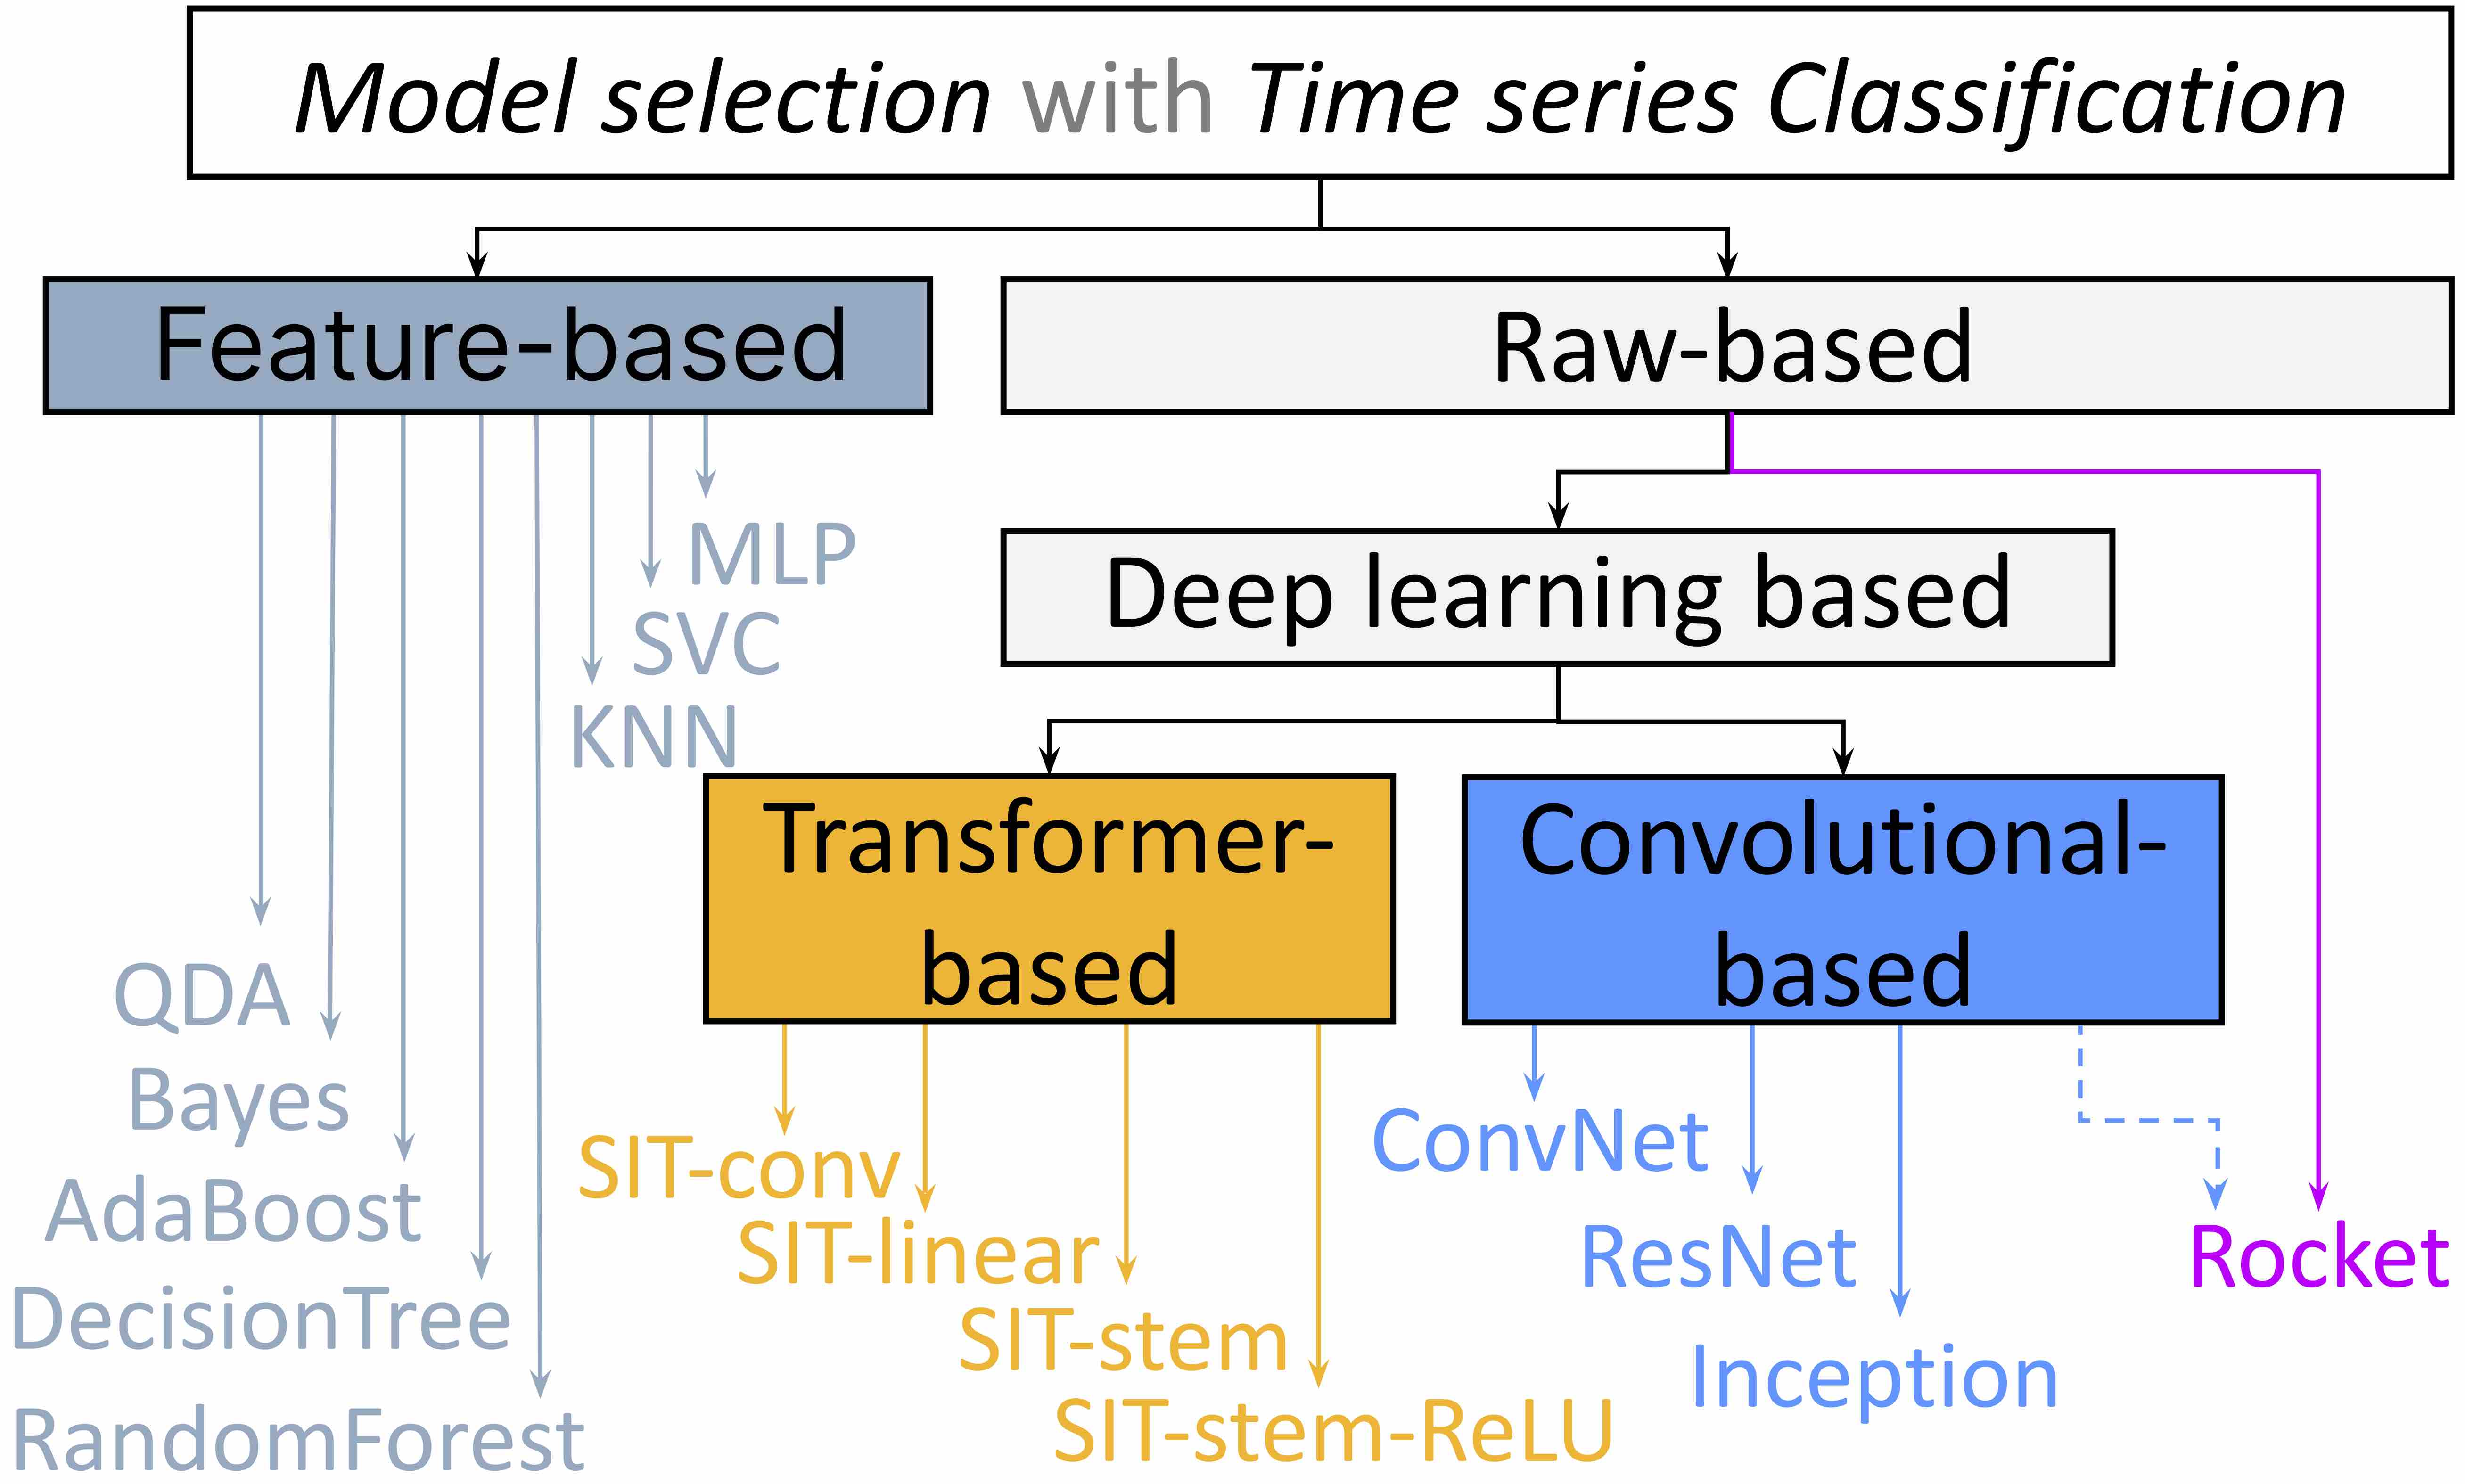
\includegraphics[width=0.76\linewidth]{figures/4_taxonomy_MS.jpg}
    \vspace{-0.3cm}
    \caption{Taxonomy of time series classification approaches used as model selection methods. We use the same color code for each class in all figures in the paper.}
    \label{fig:taxonomy}
    \vspace{-0.3cm}
\end{figure}


\subsection{Selecting the Detector}

We train the time series classification methods mentioned in the previous section to predict the best detector for each subsequence (as shown in Figure~\ref{fig:proposed_work} (c)). However, there is no guarantee that the classification model selects the same detector for all subsequences. Therefore, we choose the best detector for one time series by doing a majority voting step between the predictions for every subsequence, such that the most voted detector is selected as the detector of the time series. Formally, given a classification model $\mathcal{M}_{cl}$ applied on a given time series $T$ subsequences $\mathbb{T}_\ell$, we define $\mathcal{M}_{cl}(\mathbb{T}_\ell)$ the set of model selected for each subsequence in $\mathbb{T}_\ell$. Therefore, we define the majority voting function as follows:
\begin{equation*}
     f_{MV}(T,\mathcal{M}_{cl}) = \operatorname*{argmax}_{D \in \mathcal{M}_{cl}(\mathbb{T}_\ell)} \sum_{T_{i, \ell} \in \mathbb{T}_\ell} \mathds{1}_{[\mathcal{M}_{cl}(T_{i, \ell}) = D]}
\end{equation*}

Majority voting serves the pipeline with two significant factors, (i) it does not depend on the design of the detector and makes the pipeline easily usable for multiple different types of anomaly detection methods, and (ii) majority voting averages the predictions and reduces the impact of misclassified subsequences. To conclude, in our pipeline, the model selection method introduced in Problem~\ref{prob:probdef} is the output of $f_{MV}(T,\mathcal{M}_{cl})$.